%!TEX root = ../tese.tex
%!TEX encoding = UTF-8 Unicode
\chapter{Evaluation}\label{chapter:evaluation}
In order to evaluate the developed solution, we performed several tests to measure and evaluate the accuracy and performance of Shuttle. Due to public cloud costs, we performed a accuracy test prototype on a single machine and evaluate the prototype performance on a public \acf{CSP}.

The following sections detail the steps and decisions towards evaluating the proposed solution, starting by the definition of the developed prototype application and performed tests. The recovery accuracy and performance are evaluated on a set of intrusion scenarios. Finally, we present a cost estimation for Shuttle in \ac{AWS} \cite{aws}. The success of Shuttle is determined by its capability to recover from the intrusion scenarios in a correct, timely and scalable way.


%%%%%%%%%%%%%%%%%%%%%%%%%%%%%%%%%%%%%%%%%%%%%%%%%%%%%%%%%%%%%%%%%%%%%%%%%%%%%%%%%%%%%%%%%%%%%%%%%%%%%%%%%%%%%%%%
\section{Tests Description}\label{sec:eval:test_description}

%TryOut
We developed a \ac{HTTP} load testing and benchmarking tool, named \emph{TryOut}, to evaluate Shuttle and measure its overhead simulating a real application load from multiple clients. \emph{TryOut} consists on multiple \ac{HTTP} clients, which are deployed in various nodes, coordinated by a master node. It measures the average, minimum and maximum response time, the request rate and the throughput of each \ac{HTTP} client. \emph{TryOut} also compares the database entries and the user responses with the expected values to measure the precision and recall of our solution. TryOut allows to measure the latency for a given throughput and number of concurrent clients. Requests can be issued asynchronously or synchronously. It also allows to measure the maximum throughput supported by the service. Its main feature, comparing with tools such as Jmeter \cite{jmeter}, ab \cite{ab} and weighttp \cite{weighttp} is the capability to perform \ac{HTTP} requests based on data contained in files. This feature allows us to easily test Shuttle with a data set extracted from an application in production.

In order to use real-world data, \emph{TryOut} performs requests to the developed \acf{QA} application (Chapter \ref{sec:impl:application}) with data extracted from the \textit{Stack Exchange Data Dump} \cite{stackexchange_data}. StackExchange, which is one of the largest \ac{QA} applications and includes \textit{StackOverflow.com} \cite{stackoverflow}, is ranked 57th for traffic in the world \cite{websiteRanking}. A 24 hours window has: 36 million page loads, 148 million \ac{HTTP} requests (1712 requests per second), 267GB retrieved, 1TB sent, 334 million \ac{SQL} queries \cite{stackStatistics}. A question takes, in average, 28ms to be rendered. The architecture encompasses 1 load balancer, 2 \ac{SQL} servers, a Redis \cite{redis} (a key-value cache and store) server and 3 web servers. Their architecture scales vertically, for instance the \ac{SQL} servers have 384 GB of memory with 1.8TB of SSD storage. Since 98,82\% of the requests are read requests, the StackExchange infrastructure relies on caching.

StackExchange provides a \ac{SQL} database dump of each portal of StackExchange. We processed all dump files, a total of 60GB of text files, using MapReduce \cite{mapreduce} to extracted the questions, answers, comments and votes. We used four MapReduce jobs to process the data: group comments per answer; group answers per question; output grouped by question; output grouped sorted by time. Doing so, we obtained two files: one grouped by question, the other sorted by they. Tables \ref{tab:totalData} and \ref{tab:totalPerTopic} describe the collected data. The original data was created between 1 August 2008 and 4 May 2014 (181565797230 milliseconds or 2102 days). 
%We estimate the number of views per day considering the period between the question creation and the dump creation (4 of May 2014).

\begin{table}[ht]
\begin{minipage}[b]{0.45\linewidth}\centering
      \begin{tabular}{|p{3.3cm}|r|}
      \hline
      		                                      & \textbf{Total}  \\ \hline
          Questions                             & 8 860 649       \\ \hline
          Answers                               & 15 475 157      \\ \hline
          Comments                              & 36 486 605      \\ \hline
          Votes                                 & 70 898 355      \\ \hline
          Tags                                  & 74 205          \\ \hline
          Views                                 & 11 097 152 219  \\ \hline
          Text of questions and answers (UTF-8) & 26.76 GB        \\ \hline  
          Text of comments (UTF-8)              & 5.61 GB         \\ \hline
      \end{tabular}
    \caption{Data description}
    \label{tab:totalData}
\end{minipage}
\hspace{0.5cm}
\begin{minipage}[b]{0.45\linewidth}	\centering
      \begin{tabular}{|l|r|r|}
        \hline
          				                    & \textbf{Average} & \textbf{Std. Deviation} \\ \hline 
          Views per question          & 1252             & 6216                    \\ \hline
          Tags per question           & 1                & 1.41                    \\ \hline
          Answers per question        & 1                & 1.73                    \\ \hline
          Comments per answer         & 2                & 3.16                    \\ \hline
          Votes per answer            & 4                & 17.11                   \\ \hline
          Text per answer (UTF-8)     & 883 B        & 1133.9 B            \\ \hline
          Text per comment (UTF-8)    & 153 B       & 122.5 B           \\ \hline
          Text per question (UTF-8)   & 1477 B       & 1951.1 B            \\ \hline
      \end{tabular}
    \caption{Data description per question}
    \label{tab:totalPerTopic}
\end{minipage}
\end{table}


\begin{figure}[!htb]
  \centering
  \subfloat[][Question requests]{\resizebox{0.45\linewidth}{!}{% GNUPLOT: LaTeX picture with Postscript
\begingroup
  \makeatletter
  \providecommand\color[2][]{%
    \GenericError{(gnuplot) \space\space\space\@spaces}{%
      Package color not loaded in conjunction with
      terminal option `colourtext'%
    }{See the gnuplot documentation for explanation.%
    }{Either use 'blacktext' in gnuplot or load the package
      color.sty in LaTeX.}%
    \renewcommand\color[2][]{}%
  }%
  \providecommand\includegraphics[2][]{%
    \GenericError{(gnuplot) \space\space\space\@spaces}{%
      Package graphicx or graphics not loaded%
    }{See the gnuplot documentation for explanation.%
    }{The gnuplot epslatex terminal needs graphicx.sty or graphics.sty.}%
    \renewcommand\includegraphics[2][]{}%
  }%
  \providecommand\rotatebox[2]{#2}%
  \@ifundefined{ifGPcolor}{%
    \newif\ifGPcolor
    \GPcolorfalse
  }{}%
  \@ifundefined{ifGPblacktext}{%
    \newif\ifGPblacktext
    \GPblacktexttrue
  }{}%
  % define a \g@addto@macro without @ in the name:
  \let\gplgaddtomacro\g@addto@macro
  % define empty templates for all commands taking text:
  \gdef\gplbacktext{}%
  \gdef\gplfronttext{}%
  \makeatother
  \ifGPblacktext
    % no textcolor at all
    \def\colorrgb#1{}%
    \def\colorgray#1{}%
  \else
    % gray or color?
    \ifGPcolor
      \def\colorrgb#1{\color[rgb]{#1}}%
      \def\colorgray#1{\color[gray]{#1}}%
      \expandafter\def\csname LTw\endcsname{\color{white}}%
      \expandafter\def\csname LTb\endcsname{\color{black}}%
      \expandafter\def\csname LTa\endcsname{\color{black}}%
      \expandafter\def\csname LT0\endcsname{\color[rgb]{1,0,0}}%
      \expandafter\def\csname LT1\endcsname{\color[rgb]{0,1,0}}%
      \expandafter\def\csname LT2\endcsname{\color[rgb]{0,0,1}}%
      \expandafter\def\csname LT3\endcsname{\color[rgb]{1,0,1}}%
      \expandafter\def\csname LT4\endcsname{\color[rgb]{0,1,1}}%
      \expandafter\def\csname LT5\endcsname{\color[rgb]{1,1,0}}%
      \expandafter\def\csname LT6\endcsname{\color[rgb]{0,0,0}}%
      \expandafter\def\csname LT7\endcsname{\color[rgb]{1,0.3,0}}%
      \expandafter\def\csname LT8\endcsname{\color[rgb]{0.5,0.5,0.5}}%
    \else
      % gray
      \def\colorrgb#1{\color{black}}%
      \def\colorgray#1{\color[gray]{#1}}%
      \expandafter\def\csname LTw\endcsname{\color{white}}%
      \expandafter\def\csname LTb\endcsname{\color{black}}%
      \expandafter\def\csname LTa\endcsname{\color{black}}%
      \expandafter\def\csname LT0\endcsname{\color{black}}%
      \expandafter\def\csname LT1\endcsname{\color{black}}%
      \expandafter\def\csname LT2\endcsname{\color{black}}%
      \expandafter\def\csname LT3\endcsname{\color{black}}%
      \expandafter\def\csname LT4\endcsname{\color{black}}%
      \expandafter\def\csname LT5\endcsname{\color{black}}%
      \expandafter\def\csname LT6\endcsname{\color{black}}%
      \expandafter\def\csname LT7\endcsname{\color{black}}%
      \expandafter\def\csname LT8\endcsname{\color{black}}%
    \fi
  \fi
  \setlength{\unitlength}{0.0500bp}%
  \begin{picture}(7200.00,5040.00)%
    \gplgaddtomacro\gplbacktext{%
      \csname LTb\endcsname%
      \put(1210,1320){\makebox(0,0)[r]{\strut{} 0}}%
      \put(1210,1814){\makebox(0,0)[r]{\strut{} 2000}}%
      \put(1210,2307){\makebox(0,0)[r]{\strut{} 4000}}%
      \put(1210,2801){\makebox(0,0)[r]{\strut{} 6000}}%
      \put(1210,3294){\makebox(0,0)[r]{\strut{} 8000}}%
      \put(1210,3788){\makebox(0,0)[r]{\strut{} 10000}}%
      \put(1210,4281){\makebox(0,0)[r]{\strut{} 12000}}%
      \put(1210,4775){\makebox(0,0)[r]{\strut{} 14000}}%
      \put(552,352){\rotatebox{45}{\makebox(0,0)[l]{\strut{}01-08-2008}}}%
      \put(1064,352){\rotatebox{45}{\makebox(0,0)[l]{\strut{}01-03-2009}}}%
      \put(1655,352){\rotatebox{45}{\makebox(0,0)[l]{\strut{}01-11-2009}}}%
      \put(2236,352){\rotatebox{45}{\makebox(0,0)[l]{\strut{}01-07-2010}}}%
      \put(2755,352){\rotatebox{45}{\makebox(0,0)[l]{\strut{}01-02-2011}}}%
      \put(3338,352){\rotatebox{45}{\makebox(0,0)[l]{\strut{}01-10-2011}}}%
      \put(3924,352){\rotatebox{45}{\makebox(0,0)[l]{\strut{}01-06-2012}}}%
      \put(4440,352){\rotatebox{45}{\makebox(0,0)[l]{\strut{}01-01-2013}}}%
      \put(5027,352){\rotatebox{45}{\makebox(0,0)[l]{\strut{}01-09-2013}}}%
      \put(5608,352){\rotatebox{45}{\makebox(0,0)[l]{\strut{}01-05-2014}}}%
      \put(176,3047){\rotatebox{-270}{\makebox(0,0){\strut{}Requests}}}%
    }%
    \gplgaddtomacro\gplfronttext{%
      \csname LTb\endcsname%
      \put(5420,4594){\makebox(0,0)[r]{\strut{}Question}}%
    }%
    \gplbacktext
    \put(0,0){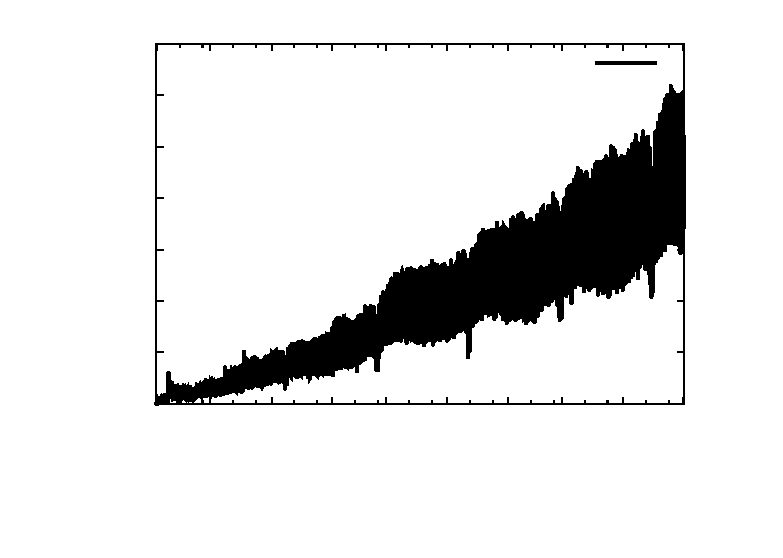
\includegraphics{graphs/requests/questions}}%
    \gplfronttext
  \end{picture}%
\endgroup
}} \quad
  \subfloat[][Answer requests]{\resizebox{0.45\linewidth}{!}{% GNUPLOT: LaTeX picture with Postscript
\begingroup
  \makeatletter
  \providecommand\color[2][]{%
    \GenericError{(gnuplot) \space\space\space\@spaces}{%
      Package color not loaded in conjunction with
      terminal option `colourtext'%
    }{See the gnuplot documentation for explanation.%
    }{Either use 'blacktext' in gnuplot or load the package
      color.sty in LaTeX.}%
    \renewcommand\color[2][]{}%
  }%
  \providecommand\includegraphics[2][]{%
    \GenericError{(gnuplot) \space\space\space\@spaces}{%
      Package graphicx or graphics not loaded%
    }{See the gnuplot documentation for explanation.%
    }{The gnuplot epslatex terminal needs graphicx.sty or graphics.sty.}%
    \renewcommand\includegraphics[2][]{}%
  }%
  \providecommand\rotatebox[2]{#2}%
  \@ifundefined{ifGPcolor}{%
    \newif\ifGPcolor
    \GPcolorfalse
  }{}%
  \@ifundefined{ifGPblacktext}{%
    \newif\ifGPblacktext
    \GPblacktexttrue
  }{}%
  % define a \g@addto@macro without @ in the name:
  \let\gplgaddtomacro\g@addto@macro
  % define empty templates for all commands taking text:
  \gdef\gplbacktext{}%
  \gdef\gplfronttext{}%
  \makeatother
  \ifGPblacktext
    % no textcolor at all
    \def\colorrgb#1{}%
    \def\colorgray#1{}%
  \else
    % gray or color?
    \ifGPcolor
      \def\colorrgb#1{\color[rgb]{#1}}%
      \def\colorgray#1{\color[gray]{#1}}%
      \expandafter\def\csname LTw\endcsname{\color{white}}%
      \expandafter\def\csname LTb\endcsname{\color{black}}%
      \expandafter\def\csname LTa\endcsname{\color{black}}%
      \expandafter\def\csname LT0\endcsname{\color[rgb]{1,0,0}}%
      \expandafter\def\csname LT1\endcsname{\color[rgb]{0,1,0}}%
      \expandafter\def\csname LT2\endcsname{\color[rgb]{0,0,1}}%
      \expandafter\def\csname LT3\endcsname{\color[rgb]{1,0,1}}%
      \expandafter\def\csname LT4\endcsname{\color[rgb]{0,1,1}}%
      \expandafter\def\csname LT5\endcsname{\color[rgb]{1,1,0}}%
      \expandafter\def\csname LT6\endcsname{\color[rgb]{0,0,0}}%
      \expandafter\def\csname LT7\endcsname{\color[rgb]{1,0.3,0}}%
      \expandafter\def\csname LT8\endcsname{\color[rgb]{0.5,0.5,0.5}}%
    \else
      % gray
      \def\colorrgb#1{\color{black}}%
      \def\colorgray#1{\color[gray]{#1}}%
      \expandafter\def\csname LTw\endcsname{\color{white}}%
      \expandafter\def\csname LTb\endcsname{\color{black}}%
      \expandafter\def\csname LTa\endcsname{\color{black}}%
      \expandafter\def\csname LT0\endcsname{\color{black}}%
      \expandafter\def\csname LT1\endcsname{\color{black}}%
      \expandafter\def\csname LT2\endcsname{\color{black}}%
      \expandafter\def\csname LT3\endcsname{\color{black}}%
      \expandafter\def\csname LT4\endcsname{\color{black}}%
      \expandafter\def\csname LT5\endcsname{\color{black}}%
      \expandafter\def\csname LT6\endcsname{\color{black}}%
      \expandafter\def\csname LT7\endcsname{\color{black}}%
      \expandafter\def\csname LT8\endcsname{\color{black}}%
    \fi
  \fi
  \setlength{\unitlength}{0.0500bp}%
  \begin{picture}(7200.00,5040.00)%
    \gplgaddtomacro\gplbacktext{%
      \csname LTb\endcsname%
      \put(1210,1320){\makebox(0,0)[r]{\strut{} 0}}%
      \put(1210,1704){\makebox(0,0)[r]{\strut{} 2000}}%
      \put(1210,2088){\makebox(0,0)[r]{\strut{} 4000}}%
      \put(1210,2472){\makebox(0,0)[r]{\strut{} 6000}}%
      \put(1210,2856){\makebox(0,0)[r]{\strut{} 8000}}%
      \put(1210,3239){\makebox(0,0)[r]{\strut{} 10000}}%
      \put(1210,3623){\makebox(0,0)[r]{\strut{} 12000}}%
      \put(1210,4007){\makebox(0,0)[r]{\strut{} 14000}}%
      \put(1210,4391){\makebox(0,0)[r]{\strut{} 16000}}%
      \put(1210,4775){\makebox(0,0)[r]{\strut{} 18000}}%
      \put(552,352){\rotatebox{45}{\makebox(0,0)[l]{\strut{}01-08-2008}}}%
      \put(1064,352){\rotatebox{45}{\makebox(0,0)[l]{\strut{}01-03-2009}}}%
      \put(1655,352){\rotatebox{45}{\makebox(0,0)[l]{\strut{}01-11-2009}}}%
      \put(2236,352){\rotatebox{45}{\makebox(0,0)[l]{\strut{}01-07-2010}}}%
      \put(2755,352){\rotatebox{45}{\makebox(0,0)[l]{\strut{}01-02-2011}}}%
      \put(3338,352){\rotatebox{45}{\makebox(0,0)[l]{\strut{}01-10-2011}}}%
      \put(3924,352){\rotatebox{45}{\makebox(0,0)[l]{\strut{}01-06-2012}}}%
      \put(4440,352){\rotatebox{45}{\makebox(0,0)[l]{\strut{}01-01-2013}}}%
      \put(5027,352){\rotatebox{45}{\makebox(0,0)[l]{\strut{}01-09-2013}}}%
      \put(5608,352){\rotatebox{45}{\makebox(0,0)[l]{\strut{}01-05-2014}}}%
      \put(176,3047){\rotatebox{-270}{\makebox(0,0){\strut{}Requests}}}%
    }%
    \gplgaddtomacro\gplfronttext{%
      \csname LTb\endcsname%
      \put(5420,4594){\makebox(0,0)[r]{\strut{}Answer}}%
    }%
    \gplbacktext
    \put(0,0){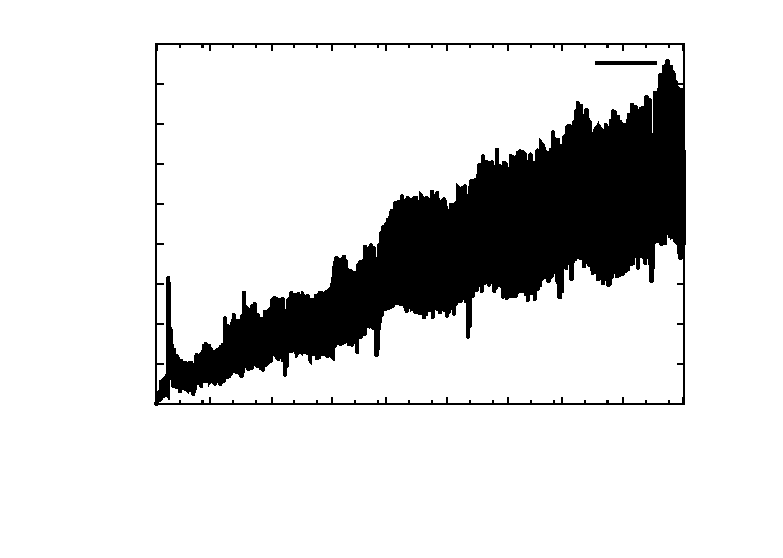
\includegraphics{graphs/requests/answers}}%
    \gplfronttext
  \end{picture}%
\endgroup
}} \\
  \subfloat[][Comment requests]{\resizebox{0.45\linewidth}{!}{% GNUPLOT: LaTeX picture with Postscript
\begingroup
  \makeatletter
  \providecommand\color[2][]{%
    \GenericError{(gnuplot) \space\space\space\@spaces}{%
      Package color not loaded in conjunction with
      terminal option `colourtext'%
    }{See the gnuplot documentation for explanation.%
    }{Either use 'blacktext' in gnuplot or load the package
      color.sty in LaTeX.}%
    \renewcommand\color[2][]{}%
  }%
  \providecommand\includegraphics[2][]{%
    \GenericError{(gnuplot) \space\space\space\@spaces}{%
      Package graphicx or graphics not loaded%
    }{See the gnuplot documentation for explanation.%
    }{The gnuplot epslatex terminal needs graphicx.sty or graphics.sty.}%
    \renewcommand\includegraphics[2][]{}%
  }%
  \providecommand\rotatebox[2]{#2}%
  \@ifundefined{ifGPcolor}{%
    \newif\ifGPcolor
    \GPcolorfalse
  }{}%
  \@ifundefined{ifGPblacktext}{%
    \newif\ifGPblacktext
    \GPblacktexttrue
  }{}%
  % define a \g@addto@macro without @ in the name:
  \let\gplgaddtomacro\g@addto@macro
  % define empty templates for all commands taking text:
  \gdef\gplbacktext{}%
  \gdef\gplfronttext{}%
  \makeatother
  \ifGPblacktext
    % no textcolor at all
    \def\colorrgb#1{}%
    \def\colorgray#1{}%
  \else
    % gray or color?
    \ifGPcolor
      \def\colorrgb#1{\color[rgb]{#1}}%
      \def\colorgray#1{\color[gray]{#1}}%
      \expandafter\def\csname LTw\endcsname{\color{white}}%
      \expandafter\def\csname LTb\endcsname{\color{black}}%
      \expandafter\def\csname LTa\endcsname{\color{black}}%
      \expandafter\def\csname LT0\endcsname{\color[rgb]{1,0,0}}%
      \expandafter\def\csname LT1\endcsname{\color[rgb]{0,1,0}}%
      \expandafter\def\csname LT2\endcsname{\color[rgb]{0,0,1}}%
      \expandafter\def\csname LT3\endcsname{\color[rgb]{1,0,1}}%
      \expandafter\def\csname LT4\endcsname{\color[rgb]{0,1,1}}%
      \expandafter\def\csname LT5\endcsname{\color[rgb]{1,1,0}}%
      \expandafter\def\csname LT6\endcsname{\color[rgb]{0,0,0}}%
      \expandafter\def\csname LT7\endcsname{\color[rgb]{1,0.3,0}}%
      \expandafter\def\csname LT8\endcsname{\color[rgb]{0.5,0.5,0.5}}%
    \else
      % gray
      \def\colorrgb#1{\color{black}}%
      \def\colorgray#1{\color[gray]{#1}}%
      \expandafter\def\csname LTw\endcsname{\color{white}}%
      \expandafter\def\csname LTb\endcsname{\color{black}}%
      \expandafter\def\csname LTa\endcsname{\color{black}}%
      \expandafter\def\csname LT0\endcsname{\color{black}}%
      \expandafter\def\csname LT1\endcsname{\color{black}}%
      \expandafter\def\csname LT2\endcsname{\color{black}}%
      \expandafter\def\csname LT3\endcsname{\color{black}}%
      \expandafter\def\csname LT4\endcsname{\color{black}}%
      \expandafter\def\csname LT5\endcsname{\color{black}}%
      \expandafter\def\csname LT6\endcsname{\color{black}}%
      \expandafter\def\csname LT7\endcsname{\color{black}}%
      \expandafter\def\csname LT8\endcsname{\color{black}}%
    \fi
  \fi
  \setlength{\unitlength}{0.0500bp}%
  \begin{picture}(7200.00,5040.00)%
    \gplgaddtomacro\gplbacktext{%
      \csname LTb\endcsname%
      \put(1210,1320){\makebox(0,0)[r]{\strut{} 0}}%
      \put(1210,1666){\makebox(0,0)[r]{\strut{} 5000}}%
      \put(1210,2011){\makebox(0,0)[r]{\strut{} 10000}}%
      \put(1210,2357){\makebox(0,0)[r]{\strut{} 15000}}%
      \put(1210,2702){\makebox(0,0)[r]{\strut{} 20000}}%
      \put(1210,3048){\makebox(0,0)[r]{\strut{} 25000}}%
      \put(1210,3393){\makebox(0,0)[r]{\strut{} 30000}}%
      \put(1210,3739){\makebox(0,0)[r]{\strut{} 35000}}%
      \put(1210,4084){\makebox(0,0)[r]{\strut{} 40000}}%
      \put(1210,4430){\makebox(0,0)[r]{\strut{} 45000}}%
      \put(1210,4775){\makebox(0,0)[r]{\strut{} 50000}}%
      \put(552,352){\rotatebox{45}{\makebox(0,0)[l]{\strut{}01-08-2008}}}%
      \put(1064,352){\rotatebox{45}{\makebox(0,0)[l]{\strut{}01-03-2009}}}%
      \put(1655,352){\rotatebox{45}{\makebox(0,0)[l]{\strut{}01-11-2009}}}%
      \put(2236,352){\rotatebox{45}{\makebox(0,0)[l]{\strut{}01-07-2010}}}%
      \put(2755,352){\rotatebox{45}{\makebox(0,0)[l]{\strut{}01-02-2011}}}%
      \put(3338,352){\rotatebox{45}{\makebox(0,0)[l]{\strut{}01-10-2011}}}%
      \put(3924,352){\rotatebox{45}{\makebox(0,0)[l]{\strut{}01-06-2012}}}%
      \put(4440,352){\rotatebox{45}{\makebox(0,0)[l]{\strut{}01-01-2013}}}%
      \put(5027,352){\rotatebox{45}{\makebox(0,0)[l]{\strut{}01-09-2013}}}%
      \put(5608,352){\rotatebox{45}{\makebox(0,0)[l]{\strut{}01-05-2014}}}%
      \put(176,3047){\rotatebox{-270}{\makebox(0,0){\strut{}Requests}}}%
    }%
    \gplgaddtomacro\gplfronttext{%
      \csname LTb\endcsname%
      \put(5420,4594){\makebox(0,0)[r]{\strut{}Comment}}%
    }%
    \gplbacktext
    \put(0,0){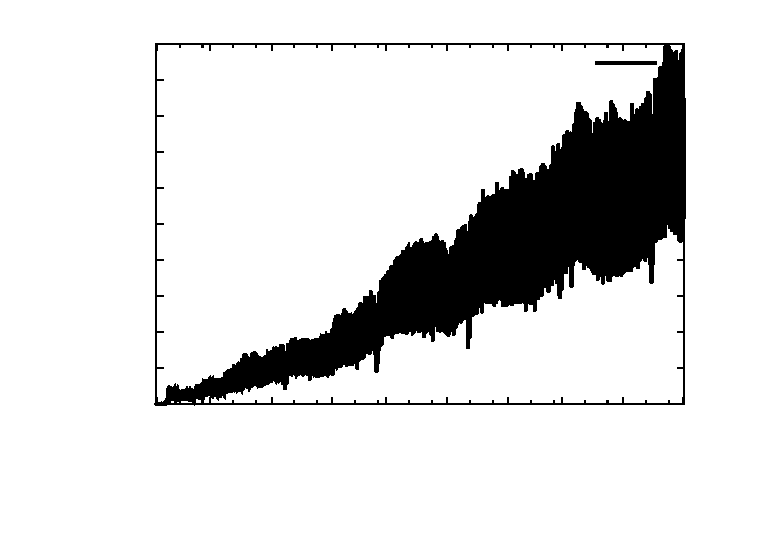
\includegraphics{graphs/requests/comments}}%
    \gplfronttext
  \end{picture}%
\endgroup
}} \quad
  \subfloat[][Vote requests]{\resizebox{0.45\linewidth}{!}{% GNUPLOT: LaTeX picture with Postscript
\begingroup
  \makeatletter
  \providecommand\color[2][]{%
    \GenericError{(gnuplot) \space\space\space\@spaces}{%
      Package color not loaded in conjunction with
      terminal option `colourtext'%
    }{See the gnuplot documentation for explanation.%
    }{Either use 'blacktext' in gnuplot or load the package
      color.sty in LaTeX.}%
    \renewcommand\color[2][]{}%
  }%
  \providecommand\includegraphics[2][]{%
    \GenericError{(gnuplot) \space\space\space\@spaces}{%
      Package graphicx or graphics not loaded%
    }{See the gnuplot documentation for explanation.%
    }{The gnuplot epslatex terminal needs graphicx.sty or graphics.sty.}%
    \renewcommand\includegraphics[2][]{}%
  }%
  \providecommand\rotatebox[2]{#2}%
  \@ifundefined{ifGPcolor}{%
    \newif\ifGPcolor
    \GPcolorfalse
  }{}%
  \@ifundefined{ifGPblacktext}{%
    \newif\ifGPblacktext
    \GPblacktexttrue
  }{}%
  % define a \g@addto@macro without @ in the name:
  \let\gplgaddtomacro\g@addto@macro
  % define empty templates for all commands taking text:
  \gdef\gplbacktext{}%
  \gdef\gplfronttext{}%
  \makeatother
  \ifGPblacktext
    % no textcolor at all
    \def\colorrgb#1{}%
    \def\colorgray#1{}%
  \else
    % gray or color?
    \ifGPcolor
      \def\colorrgb#1{\color[rgb]{#1}}%
      \def\colorgray#1{\color[gray]{#1}}%
      \expandafter\def\csname LTw\endcsname{\color{white}}%
      \expandafter\def\csname LTb\endcsname{\color{black}}%
      \expandafter\def\csname LTa\endcsname{\color{black}}%
      \expandafter\def\csname LT0\endcsname{\color[rgb]{1,0,0}}%
      \expandafter\def\csname LT1\endcsname{\color[rgb]{0,1,0}}%
      \expandafter\def\csname LT2\endcsname{\color[rgb]{0,0,1}}%
      \expandafter\def\csname LT3\endcsname{\color[rgb]{1,0,1}}%
      \expandafter\def\csname LT4\endcsname{\color[rgb]{0,1,1}}%
      \expandafter\def\csname LT5\endcsname{\color[rgb]{1,1,0}}%
      \expandafter\def\csname LT6\endcsname{\color[rgb]{0,0,0}}%
      \expandafter\def\csname LT7\endcsname{\color[rgb]{1,0.3,0}}%
      \expandafter\def\csname LT8\endcsname{\color[rgb]{0.5,0.5,0.5}}%
    \else
      % gray
      \def\colorrgb#1{\color{black}}%
      \def\colorgray#1{\color[gray]{#1}}%
      \expandafter\def\csname LTw\endcsname{\color{white}}%
      \expandafter\def\csname LTb\endcsname{\color{black}}%
      \expandafter\def\csname LTa\endcsname{\color{black}}%
      \expandafter\def\csname LT0\endcsname{\color{black}}%
      \expandafter\def\csname LT1\endcsname{\color{black}}%
      \expandafter\def\csname LT2\endcsname{\color{black}}%
      \expandafter\def\csname LT3\endcsname{\color{black}}%
      \expandafter\def\csname LT4\endcsname{\color{black}}%
      \expandafter\def\csname LT5\endcsname{\color{black}}%
      \expandafter\def\csname LT6\endcsname{\color{black}}%
      \expandafter\def\csname LT7\endcsname{\color{black}}%
      \expandafter\def\csname LT8\endcsname{\color{black}}%
    \fi
  \fi
  \setlength{\unitlength}{0.0500bp}%
  \begin{picture}(7200.00,5040.00)%
    \gplgaddtomacro\gplbacktext{%
      \csname LTb\endcsname%
      \put(1342,1320){\makebox(0,0)[r]{\strut{} 0}}%
      \put(1342,1666){\makebox(0,0)[r]{\strut{} 10000}}%
      \put(1342,2011){\makebox(0,0)[r]{\strut{} 20000}}%
      \put(1342,2357){\makebox(0,0)[r]{\strut{} 30000}}%
      \put(1342,2702){\makebox(0,0)[r]{\strut{} 40000}}%
      \put(1342,3048){\makebox(0,0)[r]{\strut{} 50000}}%
      \put(1342,3393){\makebox(0,0)[r]{\strut{} 60000}}%
      \put(1342,3739){\makebox(0,0)[r]{\strut{} 70000}}%
      \put(1342,4084){\makebox(0,0)[r]{\strut{} 80000}}%
      \put(1342,4430){\makebox(0,0)[r]{\strut{} 90000}}%
      \put(1342,4775){\makebox(0,0)[r]{\strut{} 100000}}%
      \put(684,352){\rotatebox{45}{\makebox(0,0)[l]{\strut{}01-08-2008}}}%
      \put(1182,352){\rotatebox{45}{\makebox(0,0)[l]{\strut{}01-03-2009}}}%
      \put(1758,352){\rotatebox{45}{\makebox(0,0)[l]{\strut{}01-11-2009}}}%
      \put(2324,352){\rotatebox{45}{\makebox(0,0)[l]{\strut{}01-07-2010}}}%
      \put(2829,352){\rotatebox{45}{\makebox(0,0)[l]{\strut{}01-02-2011}}}%
      \put(3398,352){\rotatebox{45}{\makebox(0,0)[l]{\strut{}01-10-2011}}}%
      \put(3968,352){\rotatebox{45}{\makebox(0,0)[l]{\strut{}01-06-2012}}}%
      \put(4471,352){\rotatebox{45}{\makebox(0,0)[l]{\strut{}01-01-2013}}}%
      \put(5042,352){\rotatebox{45}{\makebox(0,0)[l]{\strut{}01-09-2013}}}%
      \put(5608,352){\rotatebox{45}{\makebox(0,0)[l]{\strut{}01-05-2014}}}%
      \put(176,3047){\rotatebox{-270}{\makebox(0,0){\strut{}Requests}}}%
    }%
    \gplgaddtomacro\gplfronttext{%
      \csname LTb\endcsname%
      \put(5420,4594){\makebox(0,0)[r]{\strut{}Vote}}%
    }%
    \gplbacktext
    \put(0,0){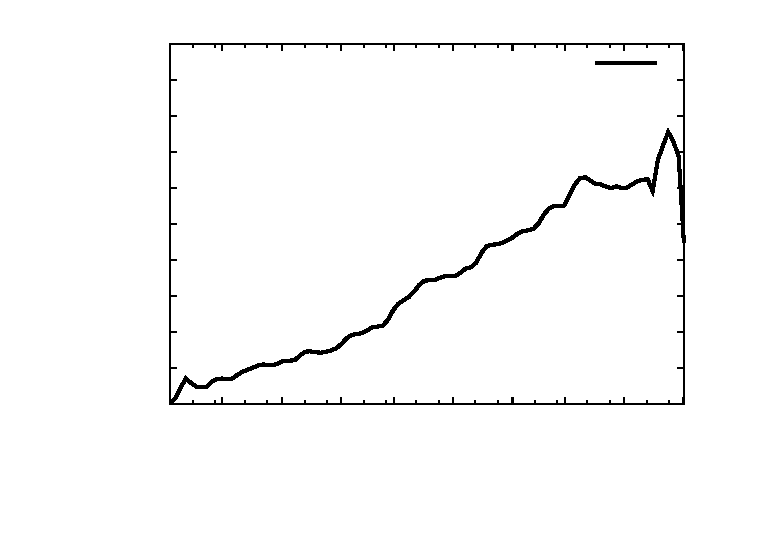
\includegraphics{graphs/requests/votes}}%
    \gplfronttext
  \end{picture}%
\endgroup
}} 
  \subfloat[][Question views]{\resizebox{0.45\linewidth}{!}{% GNUPLOT: LaTeX picture with Postscript
\begingroup
  \makeatletter
  \providecommand\color[2][]{%
    \GenericError{(gnuplot) \space\space\space\@spaces}{%
      Package color not loaded in conjunction with
      terminal option `colourtext'%
    }{See the gnuplot documentation for explanation.%
    }{Either use 'blacktext' in gnuplot or load the package
      color.sty in LaTeX.}%
    \renewcommand\color[2][]{}%
  }%
  \providecommand\includegraphics[2][]{%
    \GenericError{(gnuplot) \space\space\space\@spaces}{%
      Package graphicx or graphics not loaded%
    }{See the gnuplot documentation for explanation.%
    }{The gnuplot epslatex terminal needs graphicx.sty or graphics.sty.}%
    \renewcommand\includegraphics[2][]{}%
  }%
  \providecommand\rotatebox[2]{#2}%
  \@ifundefined{ifGPcolor}{%
    \newif\ifGPcolor
    \GPcolorfalse
  }{}%
  \@ifundefined{ifGPblacktext}{%
    \newif\ifGPblacktext
    \GPblacktexttrue
  }{}%
  % define a \g@addto@macro without @ in the name:
  \let\gplgaddtomacro\g@addto@macro
  % define empty templates for all commands taking text:
  \gdef\gplbacktext{}%
  \gdef\gplfronttext{}%
  \makeatother
  \ifGPblacktext
    % no textcolor at all
    \def\colorrgb#1{}%
    \def\colorgray#1{}%
  \else
    % gray or color?
    \ifGPcolor
      \def\colorrgb#1{\color[rgb]{#1}}%
      \def\colorgray#1{\color[gray]{#1}}%
      \expandafter\def\csname LTw\endcsname{\color{white}}%
      \expandafter\def\csname LTb\endcsname{\color{black}}%
      \expandafter\def\csname LTa\endcsname{\color{black}}%
      \expandafter\def\csname LT0\endcsname{\color[rgb]{1,0,0}}%
      \expandafter\def\csname LT1\endcsname{\color[rgb]{0,1,0}}%
      \expandafter\def\csname LT2\endcsname{\color[rgb]{0,0,1}}%
      \expandafter\def\csname LT3\endcsname{\color[rgb]{1,0,1}}%
      \expandafter\def\csname LT4\endcsname{\color[rgb]{0,1,1}}%
      \expandafter\def\csname LT5\endcsname{\color[rgb]{1,1,0}}%
      \expandafter\def\csname LT6\endcsname{\color[rgb]{0,0,0}}%
      \expandafter\def\csname LT7\endcsname{\color[rgb]{1,0.3,0}}%
      \expandafter\def\csname LT8\endcsname{\color[rgb]{0.5,0.5,0.5}}%
    \else
      % gray
      \def\colorrgb#1{\color{black}}%
      \def\colorgray#1{\color[gray]{#1}}%
      \expandafter\def\csname LTw\endcsname{\color{white}}%
      \expandafter\def\csname LTb\endcsname{\color{black}}%
      \expandafter\def\csname LTa\endcsname{\color{black}}%
      \expandafter\def\csname LT0\endcsname{\color{black}}%
      \expandafter\def\csname LT1\endcsname{\color{black}}%
      \expandafter\def\csname LT2\endcsname{\color{black}}%
      \expandafter\def\csname LT3\endcsname{\color{black}}%
      \expandafter\def\csname LT4\endcsname{\color{black}}%
      \expandafter\def\csname LT5\endcsname{\color{black}}%
      \expandafter\def\csname LT6\endcsname{\color{black}}%
      \expandafter\def\csname LT7\endcsname{\color{black}}%
      \expandafter\def\csname LT8\endcsname{\color{black}}%
    \fi
  \fi
  \setlength{\unitlength}{0.0500bp}%
  \begin{picture}(7200.00,5040.00)%
    \gplgaddtomacro\gplbacktext{%
      \csname LTb\endcsname%
      \put(1474,1320){\makebox(0,0)[r]{\strut{} 0}}%
      \put(1474,1666){\makebox(0,0)[r]{\strut{} 2e+06}}%
      \put(1474,2011){\makebox(0,0)[r]{\strut{} 4e+06}}%
      \put(1474,2357){\makebox(0,0)[r]{\strut{} 6e+06}}%
      \put(1474,2702){\makebox(0,0)[r]{\strut{} 8e+06}}%
      \put(1474,3048){\makebox(0,0)[r]{\strut{} 1e+07}}%
      \put(1474,3393){\makebox(0,0)[r]{\strut{} 1.2e+07}}%
      \put(1474,3739){\makebox(0,0)[r]{\strut{} 1.4e+07}}%
      \put(1474,4084){\makebox(0,0)[r]{\strut{} 1.6e+07}}%
      \put(1474,4430){\makebox(0,0)[r]{\strut{} 1.8e+07}}%
      \put(1474,4775){\makebox(0,0)[r]{\strut{} 2e+07}}%
      \put(816,352){\rotatebox{45}{\makebox(0,0)[l]{\strut{}01-08-2008}}}%
      \put(1301,352){\rotatebox{45}{\makebox(0,0)[l]{\strut{}01-03-2009}}}%
      \put(1861,352){\rotatebox{45}{\makebox(0,0)[l]{\strut{}01-11-2009}}}%
      \put(2412,352){\rotatebox{45}{\makebox(0,0)[l]{\strut{}01-07-2010}}}%
      \put(2904,352){\rotatebox{45}{\makebox(0,0)[l]{\strut{}01-02-2011}}}%
      \put(3457,352){\rotatebox{45}{\makebox(0,0)[l]{\strut{}01-10-2011}}}%
      \put(4012,352){\rotatebox{45}{\makebox(0,0)[l]{\strut{}01-06-2012}}}%
      \put(4502,352){\rotatebox{45}{\makebox(0,0)[l]{\strut{}01-01-2013}}}%
      \put(5057,352){\rotatebox{45}{\makebox(0,0)[l]{\strut{}01-09-2013}}}%
      \put(5608,352){\rotatebox{45}{\makebox(0,0)[l]{\strut{}01-05-2014}}}%
      \put(176,3047){\rotatebox{-270}{\makebox(0,0){\strut{}Requests}}}%
    }%
    \gplgaddtomacro\gplfronttext{%
      \csname LTb\endcsname%
      \put(5420,4594){\makebox(0,0)[r]{\strut{}Views}}%
    }%
    \gplbacktext
    \put(0,0){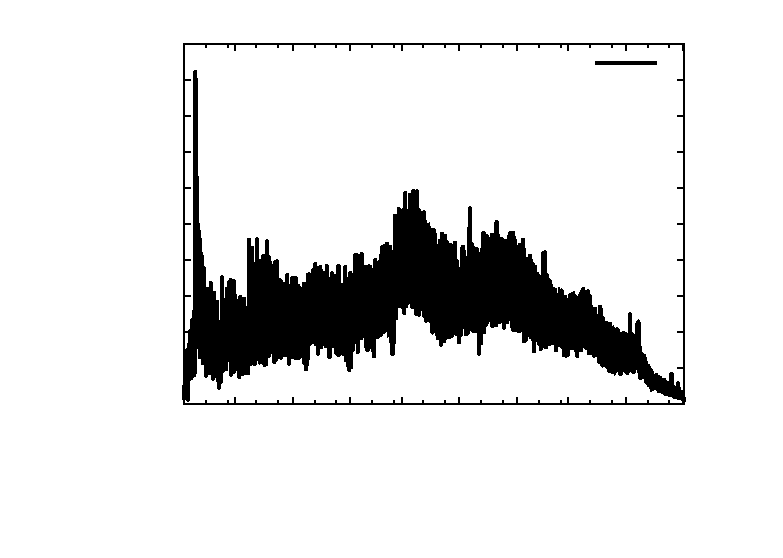
\includegraphics{graphs/requests/views}}%
    \gplfronttext
  \end{picture}%
\endgroup
}} \quad
  \caption{Number of requests per day}
  \label{fig:stackNetworkRequestRate}
\end{figure} 

The Figure \ref{fig:stackNetworkRequestRate} shows the number of new questions, answers and comments per day in the collected data during sampling period. Considering the collected data, we can set a supreme limit of 182 000 \emph{write requests} per day (2 per second if we consider a constant request rate). 

In order to set the throughput expectation for Shuttle, we assume the following request rate ranges for each category of application (Table \ref{tab:base_throughputs}). We consider small-scale applications to retrieve less than 5 million requests per day, enterprise scale retrieve between 5 and 100 million and web scale process from 100 million to billions of requests per day.
For instance, the maximum request arrival rate of one of the Portuguese Ministry of Finances web applications in 2013 was 836 requests per second and 16 million requests in total \cite{opensoft}. In contrast, the total number of requests per day of StackExchange is 148 million (1712 requests per second). We aim that Shuttle fits on current requirements for small and enterprise services. 

\begin{table}[ht]
    \centering
    \begin{tabular}{lr}
      \bf{Category}                          & \bf{Requests per day (Million)}  \\ \hline
      Small                                  & [0, 5[                           \\
      Enterprise                             & [5,100[                          \\
      Portuguese Ministry of Finances        & 16                               \\
      Web scale                              & [100,+$\infty$[                  \\
      StackExchange                          & 148                              \\
    \end{tabular}
    \caption{Throughput per web application category}
    \label{tab:base_throughputs}
\end{table}


%%%%%%%%%%%%%%%%%%%%%%%%%%%%%%%%%%%%%%%%%%%%%%%%%%%%%%%%%%%%%%%%%%%%%%%%%%%%%%%%%%%%%%%%%%%%%%%%%%%%%%%%%%%%%%%%
\section{Accuracy}\label{sec:eval:accuracy}

In this Section, we evaluate Shuttle's ability to correctly recover applications in three intrusion scenarios. \hl{diz aqui como é que fazemos essa avaliação, ou seja, resume aquilo que aparece a seguir ao longo da secção} These scenarios encompass five of the \acf{OWASP} Top 10 Application Security Risks: injection flaws, broken authentication, security misconfiguration, missing function level access control and using components with vulnerabilities \cite{Williams2013}. We consider three classes of intrusion scenarios:
\begin{itemize}
  \item Malicious requests that accidentally or maliciously compromise the application
  \item Software vulnerabilities
  \item External channels (e.g. \ac{SSH} connections)
\end{itemize}

\bigskip

We deployed all Shuttle modules, application instance and database on a single node, a 2.9GHz dual-core Intel i7 with 8GB of memory running the Java 1.7 HotSpot \acf{VM}. This configuration handled, on average, 500 requests per second from a single-thread client. We selected a subset of the \textit{StackExchange Data Dump} \cite{stackexchange_data} containing 100 000 requests originally performed from 31 of July until 12 of September of 2008: 6992 questions, 28 993 questions, 2200 comments, 61 795 votes \LONG{and 3 062 tags}. Requests were sorted per date, establishing 92 939 dependencies. For the sake of simplicity, we ignored view-only requests because the responses to every write requests imply to read the modified question.  

We considered that intrusions happen at 2nd of September, when the database contains 4338 questions, 18286 answers, 422 comments and 38334 votes (61380 requests). The attack is detected in Sep.~12th, assuming a pessimistic delay of 10 days. During this period, the application retrieved 38 620 requests.\\

Table \ref{tab:accuracy} presents a summary of the accuracy tests. It contains the number of data items tampered by the intrusion (\emph{\#intrusion}) and the number of user requests that read data items written by  tainted requests or malicious requests (without considering the intrusion requests). Recovery using \textit{full replay} requires to replay every request from the latest snapshot before the intrusion instant until the detection instant: in this example at least 38 620 requests (\emph{\#replayed (fr)}). Selective replay only re-executes tainted requests, unless some data item versions need to be recreated. On the worst case, the system does not contain any snapshot and every data read by the tainted requests shall be recreated (\emph{\#replayed (sr)}). Since Shuttle removes all the malicious actions and recovers all the legitimate requests, it has 100\% recall. The selective replay has better precision than full replay because it replays less legitimate requests.

\begin{table}
\centering
\begin{tabular}{l|rrrr}
    & \#intrusion & \#tainted & \#replayed (sr)               & \#replayed (fr)   \\ \hline
1a       & 110          & 0          & [0, 605] (18.18\%)   & > 38 620 (00.28\%)  \\
1b       & 58           & 14         & [0, 379] (18.99\%)   & > 38 620 (00.18\%)  \\
1c       & 48           & 52         & [0, 253] (39.52\%)   & > 38 620 (00.25\%)  \\
2a       & 4 338        & 0          &  -                   & > 38 620 (11.23\%)  \\
2b       & 18 286       & 1 278      &  -                   & > 38 620 (50.67\%)  \\
3        & 2 000        & -          &  -                   & > 38 620 (05.17\%)  \\
\end{tabular}
  \caption{Number of requests replayed during the recovery process and its precision within parenthesis.}
  \label{tab:accuracy}
  \vspace{-5mm}
\end{table}


%We consider an user who performed:
%Before:  2 questions, 48 answers, 0 comments, 0 votes, 1743 views
%After:  14 questions, 144 answers, 29 comments, 0 votes, 60961 views 
%Total: 16 questions, 192 answers, 29 comments, 0 votes, 62704 views 




\subsection{Result consistency}\label{sec:eval:accuracy:consistency}
%discuss what are the expectable results
Shuttle aims to support various \ac{PaaS} applications. Unlike previous works that know the application semantics \cite{undoForOperators}, the semantic of \ac{PaaS} applications is unknown to Shuttle. In order to evaluate the consistency of the results, we need to define the results expected by tenants. 

For instance, if an attacker created a new question and a legitimate user attempts to create a question with the same title. During the replay, the attacker action will be removed. Should the legitimate request be replayed and create the question? On one hand, the user may have created a question with another title but same content. On the other hand, the request contains the title that the user pretended and he may have not created another question. 

Therefore, we argue that developers should consider the application recovery during the design of the application. For instance, if questions are identified by the hash of their text instead of their title, then the legitimate users create a new question only if the text is not equal to the one of other questions. Shuttle does not replay actions which fail during their first execution. In summary, despite Shuttle's consistency \ac{API} (Section \ref{sec:arch:consistency}), developers shall take into consideration the replay process in order to obtain the expected results.\\


Considering the semantics of our \ac{QA} prototype, we identify the expected results on the following most likely attack actions:

\begin{enumerate}
  \item \textbf{Create new question:} The attacker created a new question with a specific title. The following legitimate user requests, which try to create a question with the same title, fail. When the attacker request is removed, the legitimate user requests will perform correctly and create the question. Answers to the removed question will be included in the new question.
  \item \textbf{New answer:} The attacker answer is removed correctly. Since comments to a non-existing answer fail, the comments are also removed.
  \item \textbf{New answer to every question:} Same behavior as to a new answer for a specific question.
  \item \textbf{Modify the question:} The attacker can change the title or the text. The first case is similar to create a new answer. On the second case, Shuttle loads the previous text value.
  \item \textbf{Modify the answer:} If the attacker changes the text, then Shuttle restores the previous text. However, the comments content may become inconsistent with the answer.
  \item \textbf{Delete all questions or answers:} Shuttle restores the deleted data. However, the duplicated questions and answers will fail to create.
\end{enumerate}


\subsection{Malicious Requests}\label{sec:eval:accuracy:requests}
In the first class of scenarios, we consider three cases in which an attacker has stolen an user credential. The attacker uses the stolen credential to impersonate a legitimate user and to perform malicious actions. The method used to obtain the credential is out of the scope of this dissertation. This scenario is similar to a legitimated user who makes usage mistakes.
We consider attackers:

\begin{enumerate}[label=\alph*]
  \item Deleted every question created by the user
  \item Deleted every user answer
  \item Modified every user answer
\end{enumerate}


\textit{1a)} 
%attack
The attacker deletes the user's 4 questions, performing 4 delete requests that remove 106 associated comments and answers. 
%Identify
The tenant identifies the malicious requests through the user session and selects a snapshot previous to the intrusion instant. Users cannot access deleted questions, so no request is tainted. 
%Recover using selective replay
If Shuttle has a snapshot containing the deleted questions, then \textit{selective replay} does not need to replay any request and merges the deleted questions on the current system state. If the latest snapshot is previous to the creation of the 4 questions, then \textit{selective replay} replays 605 requests to recreate the deleted questions, their answers and votes. The result is merged with the current branch, rebuilding the deleted questions. 

To clarify consider the Figure \ref{fig:attack_1_graph} in which the \emph{Req. 4} deletes a question with one answer and one comment. \emph{Req. 4} is a malicious request and the values written by it ($Q1, A1, C1$) need to be removed. If tenant selects the \emph{snapshot B}, then the items $Q1, A1, C1$ are restored to the version before the delete operation and no operation is replayed. If the tenant selects the \emph{snapshot A}, then \emph{Req.1, Req.2, Req.3} are replayed to obtain the value of the $Q1, A1, C1$. 

\begin{figure}
  \centering
  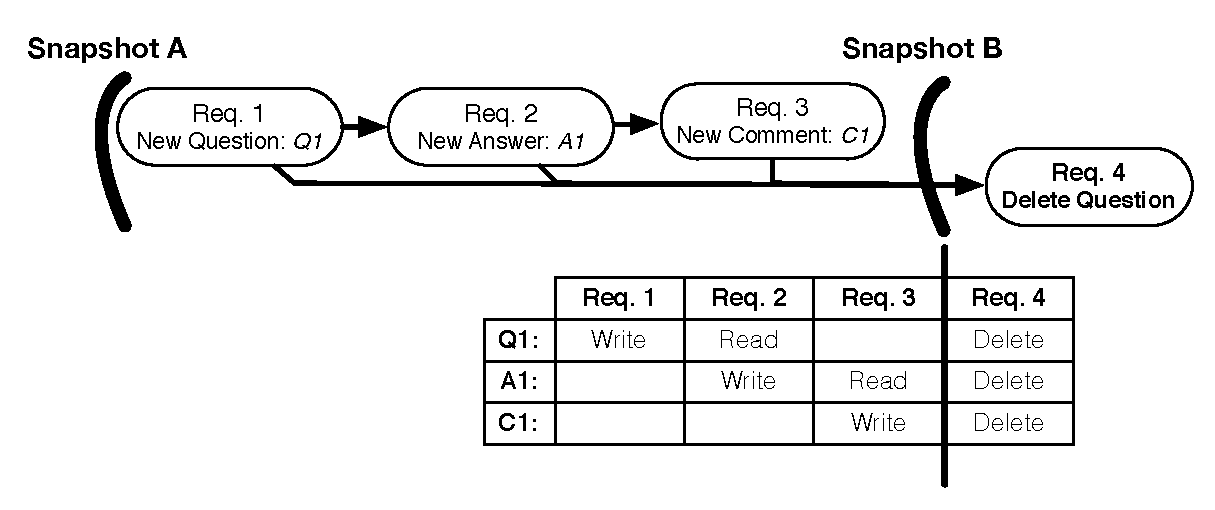
\includegraphics[width=110mm]{images/attack_1_graph}
  \caption[Example of request dependencies]{Example of request dependencies: a malicious request deletes a question with one answer and one comment}
  \label{fig:attack_1_graph}
\end{figure}

The following scenarios are similar.

\textit{1b)} Deleting the user's 48 answers implies that 58 data items are deleted and 14 answers and comments are tainted as they execute after the intrusion instant answering and voting without knowing some answers. If a snapshot containing the user answers exists, then the \textit{selective replay} approach replays only 14 tainted answers and comments. Otherwise, it replays 379 requests: the total number of requests to recreate the tainted questions and then merge the result.

\textit{1c)} 48 data items are modified while 52 requests are tainted because the users replays, votes and comments the modified questions after the intrusion instant. For recovery, the 52 tainted requests shall be replayed. If Shuttle does not have a snapshot containing the questions, then 253 requests have to be replayed to recreate them. 



%%%%%%%%%%%%%%%%%%%%%%%%%%%%%%%%%%%%%%%%%%%%%%%%%%%%%%%%%%%%%%%%%%%%%%%%%%%%%%%%%%%%%%%%%%%%%%%%%%%%%%%%%%%%%%%%%%%%%%%%%%%%%%%%%%%%%%%
\subsection{Software Vulnerability}\label{sec:eval:accuracy:software}
On the second class, we evaluate intrusion scenarios where software flaws allow attackers to modify the database without authorization. For instance, a code version added a flaw that allows \emph{SQL-Injection}. We consider two independent scenarios where the attacker:

\begin{enumerate}[label=\alph*]
  \item Deleted every question
  \item Deleted every answer
\end{enumerate}


In \textit{2a)}, the deleting of every question removes 4 338 data items. In \textit{2b)}, the questions are preserved but 1 278 answers, votes and comments are tainted as the user did not see the deleted answers.


%The attacker replaced the application version by one that accepts unauthenticated requests and stores random data items in the database. Under these circumstances, the intrusion effects are unknown.

Instead of identifying the requests that explored the vulnerability, the tenant patches the code to remove the application vulnerability. The instance rejuvenation mechanism terminates the current application instances and deploys the newest application version (Section \ref{sec:arch:image_rejuvenation}). Then, they use the \textit{full replay} to repeat all requests since the beginning of usage of the software version with the flaw. Requests that explored the vulnerability fail to execute and a consistent application state is recovered.\\

%Extra-cases: 1
Shuttle can also be used to perform preventive updates. Consider the following case: the security team considered that: a) every answer shall be ciphered using the username; b) users without weak-passwords shall not be allowed to answer questions. The development team can rapidly develop a new software version fixing these vulnerabilities. Without Shuttle the system administrator would need to create a script to make the database consistent with the new software version. Shuttle can remove these steps, which require extensive human intervention, by replaying every user request.

\subsection{External Channels}\label{sec:eval:accuracy:external}
On the third class of intrusion scenarios, we consider a case where the proxy does not log the attacker actions. In this section, we propose how to recover from a shellshock attack using Shuttle.

%Shellshock resume
Shellsock vulnerability allows an attacker to execute commands that are interpreted by the bash, i.e., perform code injection. When an attacker sends a \ac{HTTP} request containing the header \emph{User-Agent: () \{ :; \}; <malicious command>} and the web server passes this header field as a bash variable, the bash interprets the malicious command. For sake of clarity, we omit further details. In summary, this vulnerability allows a \ac{HTTP} request to run bash commands.

%Attack
We consider a case in which an attacker used an \ac{HTTP} request to create a new \ac{SSH} user account in one application server. Then, the attacker established a \ac{SSH} connection to an application server using the new user. The attacker stolen a database credentials stored in the application code. The attacker used the credentials to modify at least 2000 data items bypassing Shuttle's database proxy. As consequence, the database operations are not logged and the number of tainted requests is unknown.

%Solution
Tenants can use Shuttle as a request logger to detect the string that exploits the shellshock vulnerability: \emph{() \{:;\};}. If an intrusion is detected, the tenant selects a snapshot previous to the request creation, which does not contain data tampered by the intrusion. Since the application instances can be tampered, Shuttle uses the instance rejuvenation mechanism to terminate these instances and redeploy the application in new instances, in which the shellshock vulnerability is fixed.

%Requests are not logged
Shuttle removes the attack effects and recovers the application consistency performing \emph{full replay}. It loads a full database snapshot instead of undoing operations. As consequence, even non-logged operations are undo. Then it replays every HTTP request posterior to the snapshot instant. Since malicious actions were not logged, they are not replayed.\\

The described scenario assumes that Shuttle's trusted computing base is not compromised.

\subsection{Discussion}\label{sec:eval:accuracy:discussion}
The number of requests to replay is defined by the snapshot instant: on \textit{full replay} Shuttle replays all requests performed after the intrusion instant, while on \textit{selective replay} Shuttle replays the requests necessary to read the values of the entries before the intrusion and the tainted requests. While \textit{selective replay} seems to have a big advantage comparing with  \textit{full replay}, which performs, in these scenarios, at least 38 620 requests, most real applications have more dependencies thus the number of tainted requests is bigger. For instance, if the order between questions with the same tag is considered as a dependency,  the number of dependencies rises from 92 939 to 109 118 and the number of independent clusters decreases from 6992 to 56. We plan to further analyze the dependencies established by different types of applications.



% atacante não está logado (mas consegue fazer operações de algum modo)
% \hl{explicar bem o que é o perimetro de seguranca, o que é quebrar esse perimetro e conseguir modificar as instancias. Explicar que o Shuttle nao pode ser comprometido.}
% \textbf{Background:} The prototype \ac{QA} application displays the data that is stored in the database. In this scenario, an attacker is not logged on the application but exploits a container or application vulnerability to gain access to the Voldemort database and modifies a random set of data items without proper authorization. The database may be replicated and the application may use a byzantine fault tolerance mechanism. However, here, we ignore these mechanisms and assume a single non-replicated database.

% The attacker may create questions or answer, create an answer for every question, modify question or answer, delete all questions or answers or even randomly modify part of the database entries or delete every database entry. If the attacker actions were known, the tenant could revert them manually. However, it is arguably hard to track the attacker actions. 

% Even so, the tenant can estimate when the intrusion occurred and if the attacker used application requests or external actions. To do so, the tenant can use Shuttle not only to compare the checkpoints but also to detect database entries without associated requests. Since Shuttle keeps the records on its persistent state of the requests number that accessed each entry, if the attacker creates new entries without using the database \acAPI}, the new entries will not have a consistent sequence of requests. 

% Attacks using user requests are handled in Section \ref{sec:eval:consistency:corrupted_requests}. If the attacker used external actions, the tenant chooses a snapshot previous to the estimated intrusion moment and uses Shuttle to replay the requests after the snapshot. The external actions are not logged, thus not performed, and their effects are removed by loading the snapshot. The tenant may check the recovery process result in a separate branch before publish the results. The number of requests to replay depends only from the estimated intrusion moment and the snapshot previous to that moment. \\


% \textbf{Simulation:} To simulate this case, we executed the first \hl{XX} weeks of the StackExchange \hl{tem de dizer acima as quantidades de cada} to generate the result of an intrusion-less execution. Then, to simulate the attack, we executed the first \hl{XX} weeks and performed a set of intrusive actions directly on the database. Then, to simulate the attack effects, we performed the remaining weeks. Each attack created tampered an arbitrary set of data items of the database. Each attack was repeated 25 times, the standard deviation is presented between square brackets. 

% \textbf{Results:} The intrusion results are presented in Table \ref{fig:eval:scenarioA}.

% \begin{table}[ht]
%   \begin{tabular}{|p{2.6cm}|p{2.5cm}|p{2.5cm}|p{2.5cm}|p{2.5cm}|p{2.5cm}|p{2.5cm}}
%   \textbf{Attack}                 & \textbf{Affected Requests}  & \textbf{Number of Views} & \textbf{How many requests to repeat?} & \textbf{How many repeated?} &  \\ \cline{1-6}
%   Create question                 & The answers and same tags   &  -                       & 0                                     &  After the snapshot                   &  \\ \cline{1-6}
%   Create answer                   & The question and following answers and comments        & Same as question after the date        & 0          & After the snapshot                   &  \\ \hline
%   Create answer to every question &                   &                 &                              &                    &  \\ \cline{1-6}
%   Modify question                 &                   &                 &                              &                    &  \\ \cline{1-6}
%   Modify answer                   &                   &                 &                              &                    &  \\ \cline{1-6}
%   Delete all questions            &                   &                 &                              &                    &  \\ \cline{1-6}
%   Delete all answers              &                   &                 &                              &                    &  \\ \cline{1-6}
%   \end{tabular}
%   \caption{Results of intrusion scenario A}
%   \label{fig:eval:scenarioA}
% \end{table}

% intrusion compromised \hl{XXX}\% of entries in each store. \hl{XXXX} questions (\hl{XXX}\% of total) where affected.
% Random writes on \hl{XXX}\% of entries in each store 
% Qual o pedido antigo mais afetado?
% Quantos pedidos posteriores foram afectados? Quantas vezes foi visto o erro?
% Quantos pedidos tem de ser repetidos? Quantos foram repetidos?
% The attack compromised the actions performed by \hl{XXX} requests. The oldest affected request has been performed at \hl{XXXX December of XXXXX}. \hl{XXX}\% of the requests after that date were affected. Since Shuttle replays every action, the request replay precision is \hl{xxxxx}\%. The recall is 1 since every affected entry is repaired.

% Performing the selective replay of the affected requests, we the precision is \hl{XXXX} and the recall \hl{XXXX}. 

%The intrusions on these scenarios compromise the \ac{PaaS} containers and/or the database. Shuttle recovers from the firsts removing the compromised containers and their attached persistent storage and then launching a new container using a new clean image and deploying the application code (Section \ref{sec:arch:image_recovery}). The remaining attacks, which this section is about, involve database using external actions or using the application requests. The following sections propose different scenarios.


%15.  Qual a disponibilidade da aplicacao:  baseado no grafo anterior mas os items da base de dados sao pesados consoante o numero de views que tem: se tiverem mais views e nao estiverem disponiveis, tem mais peso do que se tiverem menos views.




%---------------------------------- damage propagation ----------------------------------
% Gráfico com a propagacao dos danos causados consante a aplicacao: uma operação é dependente de X operações com probabilidade de X. Considerando que um set de X entradas fica tainted após X entradas, como é que se propaga? Gráfico com o non-tainted vs tainted. Indicar o numero de clusters no final.

% Fazer o save de dados para evitar o redo é dificil de prever se melhora ou nao, depende do grau de indepedencia. Se for aleatorio, os pedidos rapidamente afectam toda a base de dados. xxxxxx justificar com os dados da tabela. Se os dados forem separados, tende a haver isolamento em clusters. Nesse caso, se os clusters sao grandes, entao compensa mas basta haver 1 pedido malicioso para comprometer um cluster. Nesse caso, demora mais fazer o undo selectivo do que o redo all.
